\documentclass[a4paper]{article}
\usepackage[utf8]{inputenc}

\title{AI 1103 Assignment-1}
\author{Shantanu Pandey\\ CS20BTECH11046}
\date{}
\usepackage{amsmath}
\usepackage{amssymb}
\usepackage{amsfonts}
\usepackage{nopageno}
\usepackage[margin=1in]{geometry}
\usepackage{graphicx}
\usepackage{float}
\usepackage{multicol}
\usepackage{hyperref}
\setlength{\columnsep}{0.5cm}
\setlength{\parindent}{0em}
\usepackage{color}
\usepackage{comment}
\setlength{\columnseprule}{1pt}
\def\columnseprulecolor{\color{black}}



\begin{document}
\maketitle
\noindent
Download all python codes from here

\begin{multicols*}{2}
\noindent
\fbox{%
    \parbox{0.45\textwidth}{%
        \url{https://github.com/}
    }%
    }
    
\vspace{0.3cm}
and latex-tikz codes from  

\vspace{0.3cm}  
    
\fbox{%
    \parbox{0.45\textwidth}{%
        \url{https://gi}
    }%
    }
   
\vspace{0.5cm}
\textbf{QUESTION-4.7}
\vspace{0.5cm} 

A bag consists of 10 balls each marked with
one of the digits 0 to 9. If four balls are drawn
successively with replacement from the bag,
what is the probability that none is marked
with the digit 0?

\vspace{0.5cm}
\textbf{SOLUTION}
\vspace{0.5cm} 

\vspace{0.3cm}

Let $X$ be number marked on ball drawn.
Since the balls are drawn with replacement, the trials are Bernoulli trials.
\\
So $X$ has Binomial Distribution 
\begin{equation}
    P(X=x)=\binom{n}{x}q^{n-x}p^{x} 
\end{equation} 

Here,\\

\begin{tabular}{|c|c|c|c|c|}
\hline
\textbf{Variables} & $n$ & $p$    & $q$    & $x$          \\ \hline
\textbf{Values}    & 4 & 1/10 & 9/10 & 0 \\ \hline
\end{tabular}
\\\\
Now,

\begin{align}
P(X=0) &= \binom{4}{0} \bigg(\frac{9}{10}\bigg)^{(4-0)} \bigg(\frac{1}{10}\bigg)^{0} \\
&=\frac{4!}{(4-0)! 0!} \times 1 \times \bigg(\frac{9}{10}\bigg)^{4} \\
&=\bigg( \frac{9}{10}\bigg) ^{4} \\
&= 0.6561
\end{align}
Therefore, The probability that none of ball is marked with $0$ is \textbf{0.6561}

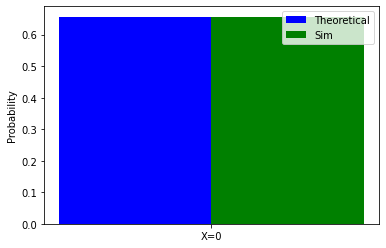
\includegraphics[scale=0.65]{Assignment1.png}\\
 The above graph shows the close relation between Theoretical and simulated results.

\end{multicols*}


\end{document}